\section{Evaluation}
The evaluation section contains three distinct components: an analysis of the performance of a few popular methods, an overview of the Kaggle predictions, and a demonstration of the Nearest Neighbor Matchup Effects.
\subsection{Popular Methods}
\andyc{Xinran's piece here}
March Madness prediction also drew attentions of many sport analysts and medias. We selected three popular predictions to examine their performances. These three models are: Nate Silver's prediction from 538.com, Ken Pomeroy's from kenpom.com and the Power Rating model from ESPN Insider. We will apply the Kaggle loss function to score these three models. As Nate Silver and Ken Pomeroy only published probabilities of each team advancing to a certain round, our comparison only considered the first round games (round of 64). \andyc{maybe include a bit little description about Ken Pom \& ESPN - could go earlier in the paper} It is also worth mentioning that the probabilities of the four teams who won their first-four games winning the round of 64 is computed as \(a/(a+b)\) where \(a\) and \(b\) are the probabilities of the team and its opponent wins.  \andyc{I know what you are doing, but it isn't clear}

The first thing to notice is that all three models concurred in all win-loss predictions of except one (Gonzaga vs OKST, 8 vs 9 in West). All three models have a similar pattern of confidence. By confidence \andyc{a different word from confidence was suggested}, we meant how far away predictions are from 0.5, e.g., predictions of 0.95 and 0.48 have confidence of 0.45 and 0.02, respectively. In all three models, most predictions either have high confidence (close to 0.5) or low confidence (close to 0 ), while moderate confidence are relatively rare. \andyc{may also be a function of the nature of first and second round games, where there are heavy favorites in many games} The reason may be a strategical adjustment for easy games. This idea may also be useful in future Kaggle competitions as to score as much as possible for easy games.

In terms of level of confidence, Silver adapted a more aggressive style than the other two. His predictions, on average, have an 0.2818 confidence while Pomeroy averages the lowest, 0.2388. However, it is showed that confidence doesn't affect the result much. For the first around games, Pomeroy has the best score of 0.4632, Silver scored 0.4664 and 0.4709 for ESPN. 

We have also examined the luck factor with these popular models. After flipping the results of five games that went overtime in round of 64, we noticed a completely reverse of the rankings of scores. The ESPN model now ranks first with 0.4631 and Pomeroy ranks third with 0.5027, Silver remains second with 0.5025. This result supported our previous conclusion that luck is a substantial factor in Kaggle. 

A further comparison showed us that the two analyst predictions are quite similar and both outperforms the ESPN model. This may be because ESPN model is strictly transitivity. Human analysts' capability of capturing intangible information regards the teams, such as  morale or playing style, could have played a vital role in avoiding transitivity and obtaining more reliable predictions. \andyc{I don't think this final sentence is true: i believe the analyst methods are data driven}

\subsection{Kaggle Leaderboard}
\andyc{is this section appropriate here?  Consider the flow of the paper the pieces come together}
\subsection{Nearest Neighbor Matchup Effects}
To demonstrate the efficacy of our method, we first fit Equation~\ref{eq:RS} using a well known rating system, the Sagarin ratings. After fitting this model, $\rho$ is calibrated based on historical results from the previous seven years NCAA tournaments. Note seven years was chosen as this is the complete history of the team level characteristics used to find neighbors of teams. The log loss for 2014 for the entire range of $\rho$ can be seen in Figure~\ref{fig:result} and the value that was selected based on historical calibration of $\rho =0.2$.
\begin{figure}[h!]
\centering
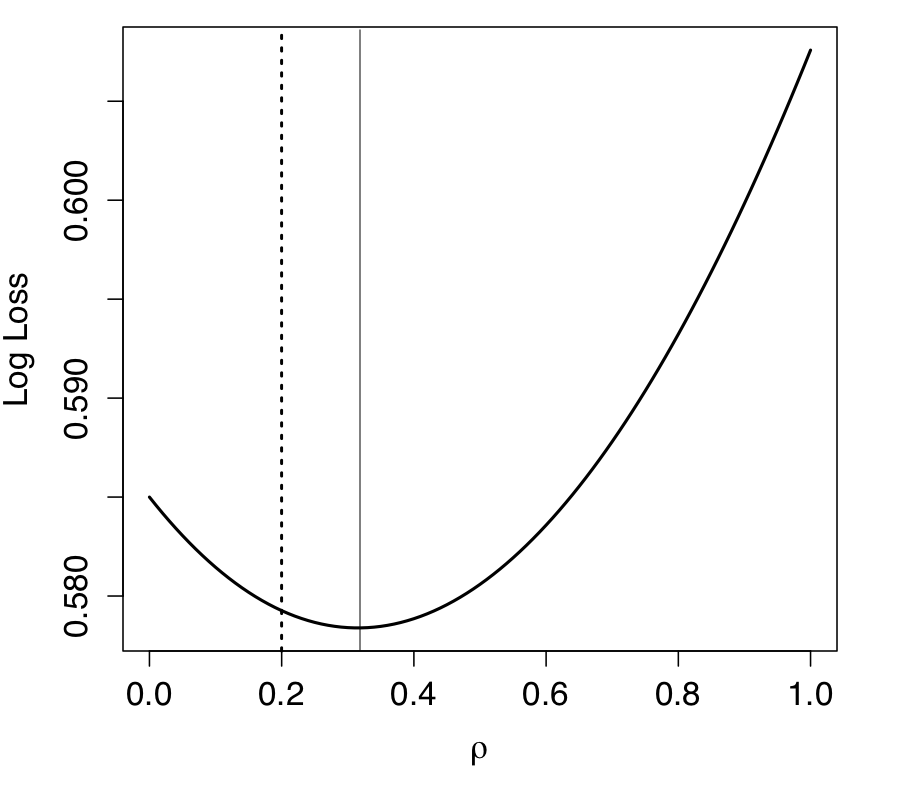
\includegraphics[width=.7\textwidth]{results_2014.png}
\caption{Log loss for no matchup effect = red, log loss for optimized $\rho$ = blue}
\label{fig:result}
\end{figure} 
\andyc{redo figure and scratch horizontal blue line} \marcosc{how past years $\rho$ on plot} \andyc{verify the quadratic nature of the plot}

The selected $\rho$ value results in a reduction in loss. A modest improvement is also seen in classification error from (0.365 to 0.350) although this is only a single game difference. The matchup effect, particularly with smaller $\rho$ values, will have a lesser effect on classification error than that of the loss functions like the log loss. This is because it will only shift the expected point differential a fairly small margin, so the only games in which classification error would change are those that are nearly dead heat games to begin with.

To illustrate the matchup effects, consider Table~\ref{tab:change} which contains the ten games that saw the largest shift in expected point differential. This table contains expected point differentials (team1 - team2) and probabilities of team 1 winning under a standard relative strength model using the Sagarin ratings as well as the adjusted results using the Nearest Neighbor Matchup Effects. The table also contains the realized loss for the each resulting game.
\begin{table}[h!]
\caption{Ten games with largest point differential change}
\tiny
\centering
\begin{tabular}{|cc | ccc | ccc | c|c|}
  \hline
  \hline
 team 1 & team 2 & Point Diff & Prob & Loss & Point Diff:ME & Prob:ME & Loss:ME & winning team &point diff\\ 
  \hline
 Cal Poly & Wichita St & -18.69 & 0.04 & 0.04 & -17.10 & 0.06 & 0.06 & Wichita St& 27\\ 
 Connecticut & St. Joseph's &4.29 & 0.65 & 0.43 & 6.18 & 0.71 & 0.34 & Connecticut & $8^*$\\ 
 Dayton & Stanford & -2.16 & 0.42 & 0.86 & 0.94 & 0.53 & 0.63 & Dayton& 10 \\ 
 Dayton & Syracuse & -6.34 & 0.28 & 1.27 & -4.05 & 0.36 & 1.03 & Dayton & 2\\ 
 Kentucky & Michigan & -3.71 & 0.37 & 1.00 & -2.08 & 0.42 & 0.86 & Kentucky & 3\\ 
 UMass & Tennessee &-3.05 & 0.39 & 0.49 & -4.83 & 0.33 & 0.40 & Tennessee &19\\ 
 Memphis & Virginia & -6.34 & 0.28 & 0.33 & -8.91 & 0.21 & 0.23 & Virginia & 18\\ 
 Michigan & Tennessee & 5.37 & 0.69 & 0.37 & 3.49 & 0.62 & 0.47 & Michigan&2\\ 
 Michigan & Texas & 8.05 & 0.77 & 0.26 & 5.85 & 0.70 & 0.35 & Michigan &14\\ 
 Syracuse & W. Michigan & 12.65 & 0.88 & 0.13 & 15.01 & 0.92 & 0.09 & Syracuse & 24\\ 
   \hline
   \hline
\end{tabular}
\label{tab:change}
\end{table}
\andyc{Include point spread?  Streamline table}
Specifically from the table, Dayton, in particular had a series of games against Syracuse and Stanford that were more favorable than a relative strength model using Sagarin would suggest. On this particular subset of games, the matchup effects model performs considerably better than the typical model under the log loss (.446 to .520). As the other games see minimal matchup effects, the results are essentially the same.  